\documentclass[border=3pt]{standalone}
% Shared TikZ styles for the Ch. 3–8 diagrams (standalone PDFs); extends the Ch. 1 palette (s1_vs_llm_common.tex).
\usepackage[T1]{fontenc}
\usepackage{lmodern}
\usepackage[english]{babel}
\usepackage{amsmath,amssymb}
\usepackage{tikz}
\usetikzlibrary{shapes.geometric,shapes.misc,positioning,fit,arrows.meta,calc,backgrounds,decorations.pathreplacing,patterns}
\definecolor{ioFill}{HTML}{F1F0EC}\definecolor{ioLine}{HTML}{52514E}
\definecolor{modFill}{HTML}{E8F1FB}\definecolor{modLine}{HTML}{2A78D6}
\definecolor{decFill}{HTML}{ECE9F7}\definecolor{decLine}{HTML}{4A3AA7}
\definecolor{postFill}{HTML}{FFF6E0}\definecolor{postLine}{HTML}{EDA100}
\definecolor{okFill}{HTML}{EAF7F1}\definecolor{okLine}{HTML}{1BAF7A}
\definecolor{badFill}{HTML}{FDECEC}\definecolor{badLine}{HTML}{E34948}
\definecolor{nmFill}{HTML}{EFEAF8}\definecolor{nmLine}{HTML}{4A3AA7}
\definecolor{loopRed}{HTML}{E34948}\definecolor{clusterLine}{HTML}{9A9890}\definecolor{ink2}{HTML}{52514E}
\definecolor{orangeA}{HTML}{EB6834}
\tikzset{
  every node/.style={font=\small, align=center},
  io/.style={trapezium, trapezium left angle=72, trapezium right angle=108, trapezium stretches body,
             draw=ioLine, fill=ioFill, thick, inner sep=3pt, minimum height=2.4em},
  model/.style={rectangle, draw=modLine, fill=modFill, very thick, inner sep=4pt, minimum height=2.4em, text width=#1},
  model/.default=3.6cm,
  post/.style={rectangle, draw=postLine, fill=postFill, very thick, inner sep=4pt, minimum height=2.2em, text width=#1},
  post/.default=3.6cm,
  data/.style={cylinder, shape border rotate=90, aspect=0.18, draw=okLine, fill=okFill, very thick, inner sep=3pt, minimum height=2.6em, text width=#1},
  data/.default=2.4cm,
  decision/.style={diamond, aspect=2.1, draw=decLine, fill=decFill, very thick, inner sep=1pt},
  outcome/.style={rounded rectangle, draw=#1, thick, inner sep=4pt, minimum height=2em},
  arrow/.style={-{Latex[length=2mm]}, thick, ioLine},
  dashedarrow/.style={-{Latex[length=2mm]}, thick, ioLine, dashed},
  loop/.style={-{Latex[length=2.4mm]}, line width=1.4pt, loopRed},
  cluster/.style={draw=clusterLine, dashed, rounded corners=3pt, inner sep=7pt},
  clusterlabel/.style={font=\small\bfseries, text=ioLine},
  note/.style={font=\footnotesize, text=ink2},
  tok/.style={rectangle, draw=ioLine, fill=ioFill, thin, inner sep=2pt, minimum height=1.6em, font=\footnotesize},
  vmark/.style={rectangle, draw=orangeA, fill=postFill, thick, inner sep=2pt, minimum height=1.6em, font=\footnotesize\ttfamily},
}

\begin{document}
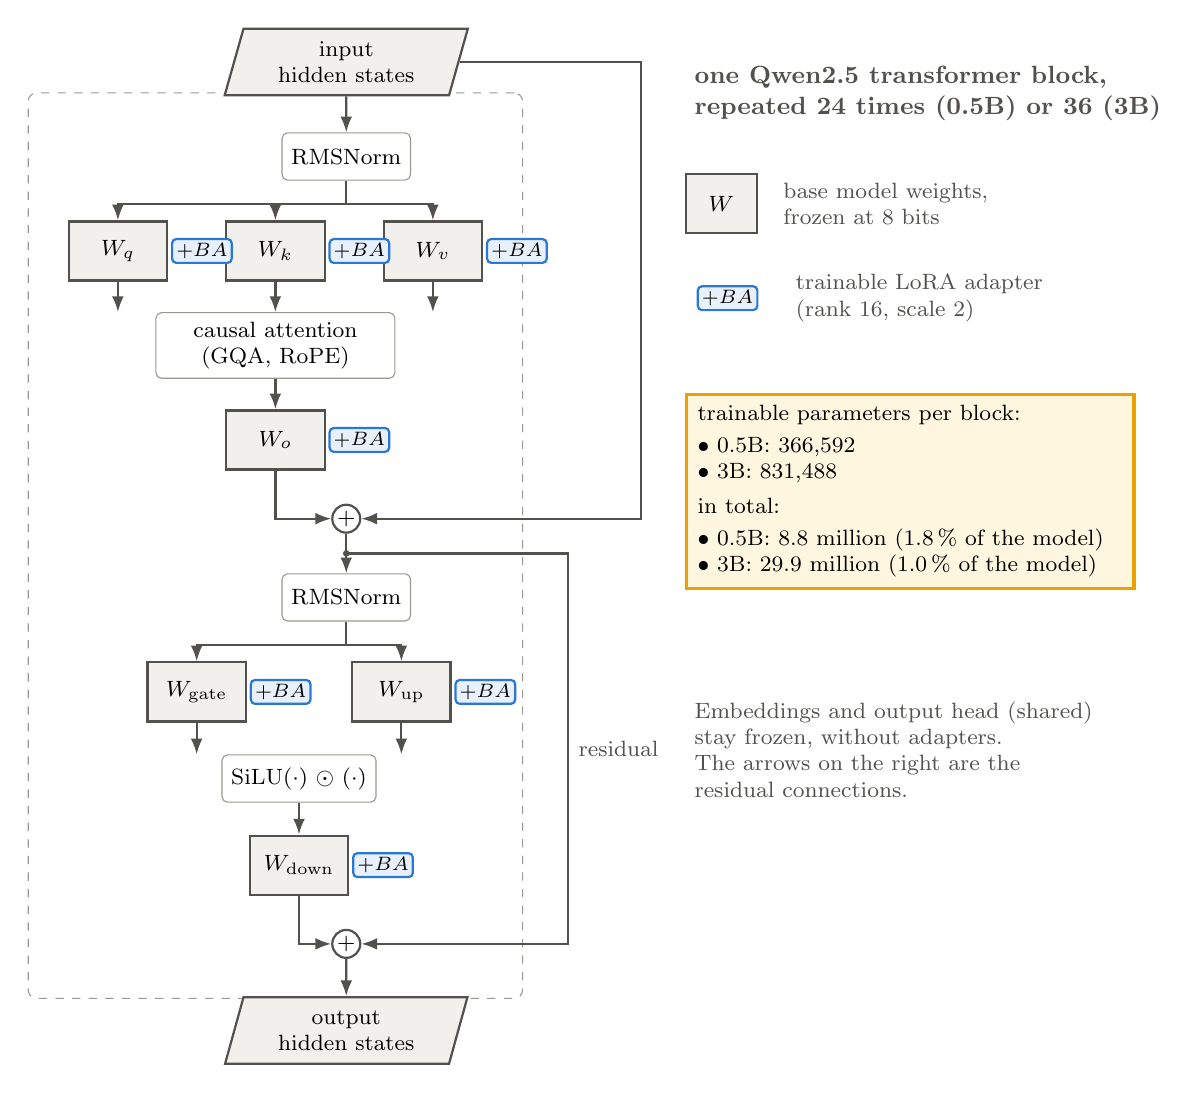
\begin{tikzpicture}[
  lin/.style={rectangle, draw=ioLine, fill=ioFill, thick, minimum width=1.25cm, minimum height=0.75cm, font=\footnotesize},
  lora/.style={rectangle, rounded corners=1.5pt, draw=modLine, fill=modFill, thick, font=\scriptsize, inner sep=1.5pt},
  op/.style={rectangle, rounded corners=2pt, draw=clusterLine, fill=white, font=\footnotesize, minimum height=0.6cm},
  sum/.style={circle, draw=ioLine, thick, inner sep=0.5pt, font=\footnotesize}]
  % input
  \node[io, text width=2.4cm, font=\footnotesize] (in) at (0,0) {input\\hidden states};
  % attention
  \node[op] (n1) at (0,-1.2) {RMSNorm};
  \node[lin] (q) at (-2.9,-2.4) {$W_q$};
  \node[lin] (k) at (-0.9,-2.4) {$W_k$};
  \node[lin] (v) at (1.1,-2.4) {$W_v$};
  \node[op, text width=2.8cm, align=center] (att) at (-0.9,-3.6) {causal attention\\(GQA, RoPE)};
  \node[lin] (o) at (-0.9,-4.8) {$W_o$};
  \node[sum] (s1) at (0,-5.8) {$+$};
  % mlp
  \node[op] (n2) at (0,-6.8) {RMSNorm};
  \node[lin] (g) at (-1.9,-8.0) {$W_\mathrm{gate}$};
  \node[lin] (u) at (0.7,-8.0) {$W_\mathrm{up}$};
  \node[op] (act) at (-0.6,-9.1) {SiLU($\cdot$) $\odot$ ($\cdot$)};
  \node[lin] (d) at (-0.6,-10.2) {$W_\mathrm{down}$};
  \node[sum] (s2) at (0,-11.2) {$+$};
  \node[io, text width=2.4cm, font=\footnotesize] (out) at (0,-12.3) {output\\hidden states};
  % LoRA badges
  \foreach \n in {q,k,v,o,g,u,d} \node[lora, anchor=west] at ([xshift=1pt]\n.east) {$+BA$};
  % arrows
  \draw[arrow] (in) -- (n1);
  \draw[arrow] (n1.south) -- ++(0,-0.3) -| (q.north);
  \draw[arrow] (n1.south) -- ++(0,-0.3) -| (k.north);
  \draw[arrow] (n1.south) -- ++(0,-0.3) -| (v.north);
  \draw[arrow] (q.south) -- (q.south |- att.north);
  \draw[arrow] (k.south) -- (att.north);
  \draw[arrow] (v.south) -- (v.south |- att.north);
  \draw[arrow] (att) -- (o);
  \draw[arrow] (o.south) |- (s1.west);
  \draw[arrow] (in.east) -- ++(2.3,0) |- (s1.east);
  \draw[arrow] (s1) -- (n2);
  \draw[arrow] (n2.south) -- ++(0,-0.3) -| (g.north);
  \draw[arrow] (n2.south) -- ++(0,-0.3) -| (u.north);
  \draw[arrow] (g.south) -- (g.south |- act.north);
  \draw[arrow] (u.south) -- (u.south |- act.north);
  \draw[arrow] (act) -- (d);
  \draw[arrow] (d.south) |- (s2.west);
  \fill[ioLine] ($(s1.south)+(0,-0.25)$) circle (1.2pt);
  \draw[arrow] ($(s1.south)+(0,-0.25)$) -- ++(2.82,0) |- (s2.east) node[pos=0.25, right, note] {residual};
  \draw[arrow] (s2) -- (out);
  % block frame
  \begin{scope}[on background layer]
    \node[cluster, fit=(n1)(q)(v)(o)(s1)(n2)(g)(u)(d)(s2), inner sep=5mm] (blk) {};
  \end{scope}
  % legend / numbers
  \node[clusterlabel, anchor=west, align=left] at (4.3,-0.4) {one Qwen2.5 transformer block,\\repeated 24 times (0.5B) or 36 (3B)};
  \node[lin, anchor=west, minimum width=0.9cm] (lw) at (4.3,-1.8) {$W$};
  \node[note, right=2mm of lw, align=left] {base model weights,\\frozen at 8 bits};
  \node[lora, anchor=west] (lb) at (4.45,-3.0) {$+BA$};
  \node[note, right=3.5mm of lb, align=left] {trainable LoRA adapter\\(rank 16, scale 2)};
  \node[post=5.4cm, font=\footnotesize, align=left, anchor=north west] at (4.3,-4.2) {trainable parameters per block:\\[2pt]
    $\bullet$ 0.5B: 366{,}592\\$\bullet$ 3B: 831{,}488\\[3pt]
    in total:\\[2pt]
    $\bullet$ 0.5B: 8.8 million (1.8\,\% of the model)\\$\bullet$ 3B: 29.9 million (1.0\,\% of the model)};
  \node[note, align=left, anchor=north west, text width=5.6cm] at (4.3,-8.0) {Embeddings and output head (shared)\\stay frozen, without adapters.\\The arrows on the right are the\\residual connections.};
\end{tikzpicture}
\end{document}
